\documentclass[border=3pt]{standalone}
% Preâmbulo compartilhado pelos diagramas TikZ da aula 11 (Localização por Grade e Monte Carlo)
\usepackage[T1]{fontenc}
\usepackage[utf8]{inputenc}
\usepackage{lmodern}
\usepackage{amsmath}
\usepackage{xcolor}
\usepackage{tikz}
\usetikzlibrary{arrows.meta,angles,quotes,decorations.pathmorphing,calc,
                positioning,shapes.geometric,shapes.misc,backgrounds,fit,
                math}

% Paleta (mesma dos SVGs originais)
\definecolor{dblue}{HTML}{2A5B8C}
\definecolor{dorange}{HTML}{B3541E}
\definecolor{dgreen}{HTML}{4A7C59}
\definecolor{dred}{HTML}{9C4B4B}
\definecolor{dcream}{HTML}{F4F1EA}
\definecolor{dshade}{HTML}{DDD7C9}

% Função gaussiana (não normalizada por padrão de escala visual)
\pgfmathdeclarefunction{gauss}{3}{%
  \pgfmathparse{1/(#3*sqrt(2*pi))*exp(-((#1-#2)^2)/(2*#3^2))}%
}

% Estilos comuns (prefixo d... para não colidir com chaves internas do pgf)
\tikzset{
  >={Stealth[length=2mm]},
  dguide/.style={gray!55, dashed, line width=0.4pt},
  daxis/.style={gray!60, line width=0.7pt, ->},
  dbody/.style={fill=black!3, draw=black!80, line width=1pt},
  dacc/.style={draw=dblue, line width=1pt},
  dlbl/.style={black!55, font=\small},
  dsub/.style={black!45, font=\footnotesize},
  dstate/.style={circle, draw=black!80, fill=dcream, line width=1pt,
                 minimum size=17mm, font=\large, inner sep=1pt},
  dobs/.style={circle, draw=black!80, fill=dshade, line width=1pt,
               minimum size=14mm, font=\large, inner sep=1pt},
  dbox/.style={rounded corners=2pt, draw=black!80, fill=dcream, line width=1pt,
               align=center, inner sep=6pt},
  dop/.style={circle, draw=black!80, fill=white, line width=1pt,
              minimum size=6mm, inner sep=0pt, font=\small},
  dtrans/.style={->, dblue, line width=1pt},
  dmeas/.style={->, dorange, line width=1pt},
  dcurve/.style={line width=1pt, dblue},
  dcurveb/.style={line width=1.4pt, dorange},
}

\begin{document}
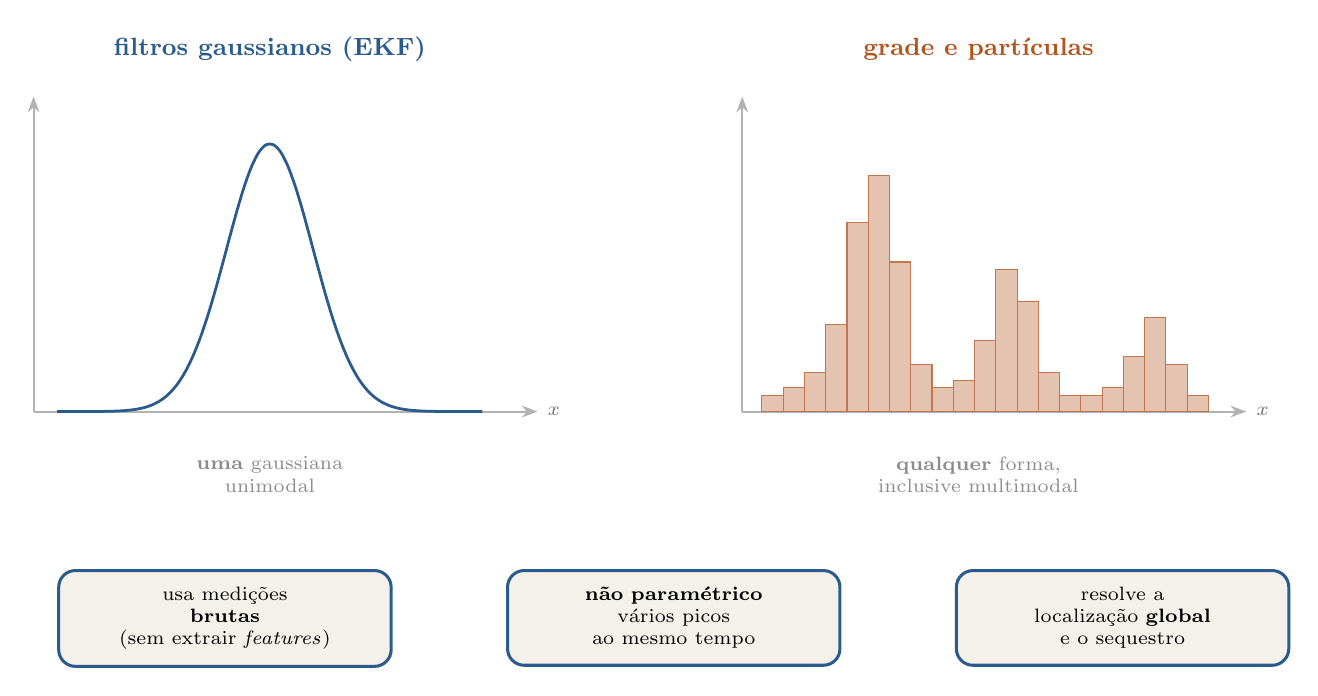
\begin{tikzpicture}[x=1cm,y=1cm]
  % painel esquerdo: gaussiana
  \node[font=\small\bfseries, dblue] at (3,4.6) {filtros gaussianos (EKF)};
  \draw[daxis] (0,0) -- (6.4,0) node[right, dlbl, font=\scriptsize] {$x$};
  \draw[daxis] (0,0) -- (0,4.0);
  \draw[dcurve, domain=0.3:5.7, samples=60, smooth] plot (\x, {3.4*exp(-((\x-3)^2)/(2*0.55^2))});
  \node[dsub, font=\scriptsize, align=center] at (3,-0.8) {\textbf{uma} gaussiana\\ unimodal};

  % painel direito: não paramétrico (histograma + partículas)
  \begin{scope}[shift={(9,0)}]
    \node[font=\small\bfseries, dorange] at (3,4.6) {grade e partículas};
    \draw[daxis] (0,0) -- (6.4,0) node[right, dlbl, font=\scriptsize] {$x$};
    \draw[daxis] (0,0) -- (0,4.0);
    \foreach \h [count=\i] in {0.2,0.3,0.5,1.1,2.4,3.0,1.9,0.6,0.3,0.4,0.9,1.8,1.4,0.5,0.2,0.2,0.3,0.7,1.2,0.6,0.2} {
      \fill[dorange!35, draw=dorange!80, line width=0.4pt] ({0.25+(\i-1)*0.27},0) rectangle ({0.25+\i*0.27},\h);
    }
    \node[dsub, font=\scriptsize, align=center] at (3,-0.8) {\textbf{qualquer} forma,\\ inclusive multimodal};
  \end{scope}

  % propriedades
  \foreach \x/\t in {0.3/{usa medições\\ \textbf{brutas}\\ (sem extrair \textit{features})}, 6.0/{\textbf{não paramétrico}\\ vários picos\\ ao mesmo tempo}, 11.7/{resolve a\\ localização \textbf{global}\\ e o sequestro}} {
    \node[dbox, rounded corners=6pt, draw=dblue, line width=1.1pt, text width=3.8cm, font=\scriptsize, anchor=north west] at (\x,-2.0) {\t};
  }
\end{tikzpicture}
\end{document}
